% ============================================================
% Artículo -- caso fútbol, HMM
% Estructura: plantilla del curso (articulo.pdf).
% Texto en rojo = \pendiente{...}: requiere decisión o ejecución.
% Resultados generados desde results/ (main_simulation.py,
% figuras.py, tablas_latex.py); ver bitacora.md.
% ============================================================
\documentclass[11pt,a4paper]{article}

\usepackage[utf8]{inputenc}
\usepackage[T1]{fontenc}
\usepackage[spanish,es-noshorthands,es-tabla]{babel}
\usepackage{lmodern}
\usepackage[margin=2.5cm]{geometry}
\usepackage{amsmath,amssymb}
\usepackage{booktabs,tabularx,array}
\usepackage{enumitem}
\usepackage{xcolor}
\usepackage{graphicx}
\usepackage{adjustbox}
\usepackage{url}
\setlength{\emergencystretch}{3em}
\usepackage{listings}
\usepackage[hidelinks]{hyperref}

\newcommand{\pendiente}[1]{\textcolor{red}{\textbf{[Pendiente: #1]}}}
\DeclareMathOperator*{\argmax}{arg\,max}

\lstset{
  language=Python, basicstyle=\ttfamily\small, numbers=left,
  numberstyle=\tiny, frame=single, breaklines=true,
  keywordstyle=\color{blue!60!black}, commentstyle=\color{gray},
  columns=fullflexible
}

\title{Aporte de la dependencia temporal a la inferencia de fases tácticas
simuladas mediante Modelos Ocultos de Markov}

\author{
Juan Sebastian Lopez Gallo$^{1}$, Andres Miguel Hernandez$^{1}$\\[4pt]
\small $^{1}$Ingeniería de Software y Datos, IU Digital. Curso: Simulación\\
\small Correo electrónico: js.lopez.academic.2003@gmail.com,\
andres.hernandez74@est.iudigital.edu.co\\
\small Docente: Julian Andres Loaiza Lopez
}

\date{9 de noviembre de 2026}

\begin{document}
\maketitle

% ------------------------------------------------------------
\begin{abstract}
La fase táctica de un equipo de fútbol (defensiva, transición, ataque) no se
observa directamente; solo se observan acciones con balón, y una acción aislada
no determina la fase. Mediante simulación controlada con un Modelo Oculto de
Markov (HMM) de parámetros hipotéticos conocidos, se evaluó cuánto aporta la
dependencia temporal a la inferencia de esas fases. Se compararon la
decodificación de Viterbi y la decodificación posterior (forward--backward) con
un clasificador que asigna a cada acción la fase más probable sin considerar
transiciones, usando la exactitud por paso frente a la fase simulada en nueve
configuraciones (parámetros del caso, emisiones más ambiguas y transiciones
menos persistentes), con 100 réplicas por configuración. Con los parámetros del
caso, Viterbi fue menos exacto que el clasificador sin transiciones (diferencia
media $-0.033$; IC95\,\% $[-0.034,\,-0.031]$), mientras que la decodificación
posterior lo superó por un margen pequeño ($+0.002$; IC95\,\%
$[+0.0016,\,+0.0025]$). Con emisiones más ambiguas, Viterbi terminó asignando una
sola fase; con transiciones menos persistentes, los tres métodos produjeron
asignaciones idénticas a partir de cierto nivel. Los resultados se limitan al
modelo simulado y no permiten afirmaciones sobre partidos reales.
\end{abstract}

\noindent\textbf{Palabras clave:} Modelos Ocultos de Markov, algoritmo de Viterbi,
simulación, fases tácticas, fútbol, reproducibilidad.

% ------------------------------------------------------------
\section{Introducción}

Muchos fenómenos deportivos se describen como una sucesión de fases que no se
registran directamente. En fútbol, expresiones como ``fase defensiva'' o
``fase de ataque'' aluden a estados del juego que solo se manifiestan a través
de acciones observables. Los HMM ofrecen un marco probabilístico para relacionar
una secuencia de observaciones con una secuencia de estados latentes.

Ötting, Langrock y Maruotti modelan estadísticas minuto a minuto de la
Bundesliga con HMM y obtienen estados que interpretan como distintos niveles de
control del partido \cite[pp.~9, 20]{otting2023}. Los mismos autores advierten
que, en un ajuste no supervisado, los estados de un HMM son solo aproximaciones
de estados genuinos y que la secuencia decodificada puede diferir de la real
\cite[p.~23]{otting2023}. Esa advertencia motiva el presente trabajo: antes de
interpretar estados latentes en datos reales, conviene saber cuánto puede
recuperar un HMM en condiciones donde la verdad sí se conoce. En otro contexto,
Fani et al.\ usan un HMM sobre la secuencia de tipos de plano de vídeos
retransmitidos para segmentar el partido en juego e interrupción, estimando los
parámetros a partir de secuencias con etiquetas de referencia
\cite[pp.~27324, 27329--27330]{fani2017}.

\subsection{Planteamiento del problema y justificación}

Con datos simulados a partir de un HMM de parámetros conocidos, no sabemos
cuánto mejora la inferencia de fases tácticas latentes cuando se usa la
dependencia temporal entre acciones, frente a clasificar cada acción por
separado, ni cómo varía esa mejora con la ambigüedad de las emisiones y la
persistencia de las fases.

El estudio se apoya en los siguientes supuestos explícitos:
\begin{enumerate}[label=S\arabic*.]
  \item Existen exactamente tres fases (defensiva, transición, ataque),
        mutuamente excluyentes. Es un supuesto del caso, no un hecho demostrado.
  \item La fase actual depende solo de la anterior (Markov de primer orden) y
        las transiciones son homogéneas en el tiempo.
  \item La acción observada depende solo de la fase actual.
  \item Tres tipos de acción (pase corto, pase largo, tiro a puerta) bastan para
        el modelo; se omiten posición, tiempo, rival y marcador.
  \item La duración en cada fase es geométrica (consecuencia de S2).
  \item La unidad de análisis es una secuencia simulada de $T=100$ acciones.
        La definición operativa de las fases y de la unidad de secuencia para
        un estudio con datos reales queda como trabajo futuro
        (sección~\ref{sec:conclusiones}, punto ii).
\end{enumerate}

\subsection{Preguntas de investigación}

\begin{description}[leftmargin=1.2cm]
  \item[P1:] Con parámetros conocidos, ¿la decodificación de Viterbi recupera
  la fase simulada con mayor exactitud por paso que un clasificador que asigna a
  cada acción la fase más probable sin considerar transiciones?
  \item[P2:] ¿Cómo varía la diferencia de exactitud entre ambos métodos cuando
  las emisiones $B$ se vuelven más ambiguas, manteniendo $A$ y $\pi$ fijos?
  \item[P3:] ¿Cómo varía esa diferencia cuando las transiciones $A$ se vuelven
  menos persistentes, manteniendo $B$ y $\pi$ fijos?
\end{description}

Ninguna pregunta presupone la superioridad del HMM: una diferencia nula o
pequeña es una respuesta válida.

\subsection{Objetivos y aportes previstos}

\textbf{Objetivo general.} Evaluar, en simulación controlada, el aporte de la
dependencia temporal de un HMM a la inferencia de fases tácticas supuestas a
partir de acciones con balón.

\textbf{Objetivos específicos.}
\begin{enumerate}
  \item Comparar la exactitud por paso de Viterbi con la de un clasificador sin
        transiciones usando los parámetros hipotéticos del caso (P1).
  \item Medir cómo cambia esa diferencia al aumentar la ambigüedad de $B$ (P2).
  \item Medir cómo cambia esa diferencia al reducir la persistencia de $A$ (P3).
\end{enumerate}

\textbf{Aportes previstos.}
(i) Una formalización del caso como $\lambda=(S,V,A,B,\pi)$ con supuestos
explícitos; (ii) un diseño experimental con comparación pareada frente a un
clasificador de referencia; (iii) código con semillas registradas y distintas
por réplica.

% ------------------------------------------------------------
\section{Estado del arte}

\textbf{Protocolo.} Por decisión del equipo, en esta fase el estado del arte se
limita a dos fuentes aportadas por el equipo: \cite{otting2023} (acceso
abierto, licencia CC BY 4.0) y \cite{fani2017} (IEEE; se cita y parafrasea sin
reproducir figuras ni tablas). Se leyó el texto completo de ambas; las tablas de
\cite{fani2017} son imágenes y no se extrajeron, por lo que solo se usan las
cifras que aparecen en su texto. No se realizó una búsqueda sistemática; por
tanto, este apartado \emph{no} permite afirmar qué existe o no existe en la
literatura. El equipo decidió no ampliarlo en esta versión porque la mayoría
de los documentos localizados eran de pago.

\begin{table}[ht]
\centering
\caption{Comparación entre las fuentes revisadas y el trabajo propuesto.}
\label{tab:sota}
\footnotesize
\begin{tabularx}{\textwidth}{>{\raggedright\arraybackslash}p{2.3cm}
  >{\raggedright\arraybackslash}X >{\raggedright\arraybackslash}X
  >{\raggedright\arraybackslash}X}
\toprule
 & Ötting et al.\ \cite{otting2023} & Fani et al.\ \cite{fani2017} & Este trabajo \\
\midrule
Pregunta & Cambios de dinámica (\emph{momentum}) dentro del partido (p.~9) &
Segmentar vídeo retransmitido en juego e interrupción (p.~27322) &
Aporte de la dependencia temporal a la inferencia de fases \\
Datos & Reales: estadísticas minuto a minuto de un equipo, 34 partidos, 3214
observaciones (p.~10) & Reales: 10 vídeos (9~h), 3452 planos (p.~27330) &
Simulados desde un HMM de parámetros conocidos \\
Observaciones & Conteos por minuto: tiros y toques de balón (p.~10) &
Tipo de plano y marca de repetición de cada plano (p.~27329) &
Acción por evento: pase corto, pase largo, tiro \\
Estados & 3, elegidos por AIC/BIC e interpretabilidad; niveles de control
(pp.~19--20) & 2: juego e interrupción (p.~27329) &
3, fijados por el caso: defensiva, transición, ataque \\
Parámetros & Estimados sin etiquetas, por máxima verosimilitud con varios
valores iniciales (pp.~14--15) & Estimados con etiquetas de referencia más un
1\,\% de ruido por iteración (p.~27330) & Conocidos; no se estiman \\
Decodificación & Viterbi (p.~22) & Viterbi, iterando con los estados inferidos
de los planos vecinos como observaciones (pp.~27329--27330) &
Viterbi frente a un clasificador sin transiciones \\
Evaluación & Ajuste (AIC, BIC) e interpretación; no hay estado verdadero
disponible & Exactitud frente a las etiquetas; 98,7\,\% para el H2O-MM, comparado
con dos HMM previos (pp.~27322, 27333) & Exactitud por paso y por fase frente a
la fase simulada; diferencia pareada con IC95\,\% \\
Limitaciones & Declaradas: estados como aproximaciones; no se separa táctica de
\emph{momentum}; un solo equipo (pp.~23--25) & Observada por nosotros: en lo
leído no se describe partición entrenamiento/prueba para el H2O-MM (pp.~27330,
27333) & Validez limitada al modelo simulado \\
\bottomrule
\end{tabularx}
\end{table}

\subsection{Relación con las fuentes y alcance de la contribución}

Las dos fuentes ilustran dos maneras de usar un HMM en fútbol. En
\cite{otting2023} los estados no tienen etiqueta: se interpretan a posteriori y
los autores advierten que solo aproximan estados genuinos
\cite[p.~23]{otting2023}. En \cite{fani2017} los estados sí tienen etiqueta, lo
que permite medir exactitud; el modelo usa contexto temporal (transiciones y,
en el H2O-MM, los estados de los planos vecinos) y se compara con otros HMM
\cite[pp.~27329--27333]{fani2017}. En los pasajes leídos, ninguna de las dos
fuentes aísla cuánto aporta la dependencia temporal frente a un clasificador
que trata cada observación por separado; esa es la cuestión que aborda este
trabajo, en un entorno simulado donde la fase verdadera se conoce. No se
afirma la existencia de un vacío en la literatura, pues dos fuentes no lo
permiten.

Dos precauciones: (i) ni los niveles de control de \cite{otting2023} (p.~20)
ni los estados juego/interrupción de \cite{fani2017} equivalen a las fases de
este caso; (ii) la exactitud de \cite{fani2017} no es comparable con la que se
obtenga aquí, porque los datos, las observaciones y el número de estados son
distintos y porque, en lo leído, no consta que se evaluara con datos separados
de los de estimación.

% ------------------------------------------------------------
\section{Marco teórico}

\subsection{Distribución de las emisiones}
Las observaciones son categóricas, $O_t\in V=\{v_1,v_2,v_3\}$ = \{pase corto,
pase largo, tiro a puerta\}. Dado el estado, la emisión sigue una distribución
categórica con probabilidades dadas por una fila de $B$.

\subsection{Propiedad de Markov}
La secuencia de fases $\{S_t\}_{t=1}^{T}$ satisface
\begin{equation}
P(S_t=s_j\mid S_{t-1}=s_i,S_{t-2},\dots,S_1)=P(S_t=s_j\mid S_{t-1}=s_i).
\end{equation}

\subsection{Formalización del HMM del caso}
El modelo es la tupla $\lambda=(S,V,A,B,\pi)$ con
$S=\{s_1,s_2,s_3\}$ = \{defensiva, transición, ataque\},
\begin{align}
a_{ij}&=P(S_t=s_j\mid S_{t-1}=s_i), & \textstyle\sum_j a_{ij}&=1,\\
b_j(k)&=P(O_t=v_k\mid S_t=s_j), & \textstyle\sum_k b_j(k)&=1,\\
\pi_i&=P(S_1=s_i), & \textstyle\sum_i \pi_i&=1.
\end{align}
Los valores hipotéticos del caso (no estimados con partidos reales) son:
\begin{equation}
A=\begin{pmatrix}0.60&0.30&0.10\\0.30&0.40&0.30\\0.20&0.30&0.50\end{pmatrix},\quad
B=\begin{pmatrix}0.70&0.25&0.05\\0.40&0.50&0.10\\0.30&0.30&0.40\end{pmatrix},\quad
\pi=(0.40,\,0.40,\,0.20).
\end{equation}
Filas de $A$: estado de origen; columnas: estado de destino. Filas de $B$:
estado; columnas: pase corto, pase largo, tiro. Se verificó que todas las filas
y $\pi$ suman 1. La distribución estacionaria de $A$ es
$p\approx(0.389,\,0.333,\,0.278)$ y las duraciones esperadas en cada fase,
$1/(1-a_{ii})$, son $2.5$, $1.67$ y $2.0$ pasos (propiedades del modelo
hipotético, no del fútbol real).

\subsection{Los tres problemas clásicos}
Con un HMM se plantean habitualmente tres tareas: evaluar la verosimilitud de
una secuencia observada, decodificar los estados ocultos y estimar los
parámetros. Ötting et al.\ usan las tres en su análisis
\cite[pp.~14--15, 22]{otting2023}; aquí se describen en la forma que emplea
este trabajo.

\begin{enumerate}
\item \textbf{Evaluación (Forward).} Calcula $P(O\mid\lambda)$ con
$\alpha_1(i)=\pi_i b_i(o_1)$ y
$\alpha_{t+1}(j)=\big[\sum_i\alpha_t(i)a_{ij}\big]b_j(o_{t+1})$,
con coste $O(TN^2)$ \cite[p.~14]{otting2023}. No responde qué fase hubo en cada
paso.
\item \textbf{Decodificación (Viterbi).} Obtiene la secuencia de estados más
probable $Q^*=\argmax_Q P(Q\mid O,\lambda)$. En log-espacio:
\begin{equation}
\delta_1(i)=\log\pi_i+\log b_i(o_1),\qquad
\delta_t(j)=\max_i\big[\delta_{t-1}(i)+\log a_{ij}\big]+\log b_j(o_t).
\end{equation}
con coste $O(TN^2)$ \cite[p.~22]{otting2023}. Es el método evaluado en este
trabajo.

\emph{Decodificación posterior (forward--backward).} Combina la variable forward
$\alpha_t(i)$ con la backward $\beta_t(i)=P(o_{t+1},\dots,o_T\mid S_t=s_i,\lambda)$
para elegir en cada paso la fase de mayor probabilidad posterior:
\begin{equation}
\hat s_t=\argmax_i\;P(S_t=s_i\mid O,\lambda)=\argmax_i\;\alpha_t(i)\,\beta_t(i).
\end{equation}
A diferencia de Viterbi, maximiza el número esperado de pasos acertados, no la
probabilidad del camino completo, por lo que la secuencia resultante puede
contener transiciones poco probables. Se implementa con factores de escala para
evitar el desbordamiento inferior. Se incorpora como método complementario
(decisión del equipo tras observar los resultados de Viterbi).
\item \textbf{Aprendizaje (Baum--Welch).} Estima $\lambda$ a partir de las
observaciones mediante EM. Ötting et al.\ estiman los parámetros de otra forma,
maximizando numéricamente la verosimilitud con 50 valores iniciales aleatorios
para evitar máximos locales \cite[pp.~14--15]{otting2023}. \emph{Queda fuera
del alcance}: aquí los parámetros son conocidos.
\end{enumerate}

\subsection{Clasificador de referencia sin transiciones}
Para aislar el efecto de la dependencia temporal, el clasificador de referencia
usa la misma información que el HMM salvo las transiciones:
\begin{equation}
\hat s_t=\argmax_i\; p_i\, b_i(o_t),
\end{equation}
donde $p$ es la distribución estacionaria de $A$. Con los parámetros del caso
asigna pase corto $\to$ defensiva, pase largo $\to$ transición y tiro $\to$
ataque.

% ------------------------------------------------------------
\section{Metodología e implementación}

\begin{table}[ht]
\centering
\caption{Fases del proyecto (F1--F7 de la plantilla) y su estado.}
\small
\begin{tabularx}{\textwidth}{l>{\raggedright\arraybackslash}X>{\raggedright\arraybackslash}X l}
\toprule
Fase & Actividad & Entregable & Estado \\
\midrule
F1 & Planteamiento del problema & Preguntas P1--P3 y alcance & Borrador \\
F2 & Revisión de literatura & Tabla~\ref{tab:sota} (dos fuentes) & Limitada \\
F3 & Diseño formal del modelo & Tupla $\lambda$ del caso & Borrador \\
F4 & Implementación & Viterbi, decodificación posterior y clasificador de referencia & Verificado$^{a}$ \\
F5 & Simulación controlada & Secuencias de E1--E3 & Ejecutada \\
F6 & Análisis estadístico & Medias, desviaciones, IC95\,\% & Hecho \\
F7 & Comunicación & Manuscrito, repositorio, vídeo & Pendiente \\
\bottomrule
\multicolumn{4}{l}{\footnotesize $^{a}$Comparados con enumeración exhaustiva en
secuencias cortas; no es un resultado experimental.}
\end{tabularx}
\end{table}

\subsection{Flujo experimental}
Para cada escenario $e\in\{\mathrm{E1},\mathrm{E2},\mathrm{E3}\}$ y cada
réplica $r=1,\dots,R$:
\begin{enumerate}
\item Generar con una semilla propia de la réplica $S$ secuencias de longitud
$T$ (fases verdaderas y acciones) desde $\lambda_e$.
\item Decodificar cada secuencia con Viterbi, con la decodificación posterior y
con el clasificador de referencia, usando los parámetros verdaderos $\lambda_e$.
\item Calcular la exactitud por paso de cada método y su diferencia pareada.
\end{enumerate}
Finalmente, resumir las $R$ réplicas por escenario.

\subsection{Pseudocódigo de Viterbi en log-espacio}

\begin{lstlisting}[caption={Viterbi en log-espacio para un HMM discreto.}]
import numpy as np

def viterbi_log(obs, A, B, pi):
    logA, logB, logpi = np.log(A), np.log(B), np.log(pi)
    N, T = A.shape[0], len(obs)
    delta = np.empty((T, N))
    psi = np.zeros((T, N), dtype=int)
    delta[0] = logpi + logB[:, obs[0]]                  # inicializacion
    for t in range(1, T):                               # recursion
        scores = delta[t-1][:, None] + logA             # scores[i, j]
        psi[t] = np.argmax(scores, axis=0)
        delta[t] = scores[psi[t], np.arange(N)] + logB[:, obs[t]]
    q = np.empty(T, dtype=int)                          # reconstruccion
    q[-1] = np.argmax(delta[-1])
    for t in range(T-2, -1, -1):
        q[t] = psi[t+1, q[t+1]]
    return q, delta[-1].max()
\end{lstlisting}

A diferencia del pseudocódigo de la plantilla, se trabaja con
log-probabilidades para evitar el desbordamiento inferior en secuencias largas.
El código completo (Viterbi, decodificación posterior, clasificador de
referencia y simulador) está en \texttt{src/hmm\_core.py}; Viterbi y la
decodificación posterior coincidieron con la enumeración exhaustiva en 100 de
100 secuencias cortas cada uno (\texttt{verificacion/}).

\subsection{Diseño experimental}

\textbf{Escenarios} (un factor controlado por escenario):
\begin{itemize}
\item \textbf{E1 (caso):} $A$, $B$, $\pi$ del caso.
\item \textbf{E2 (emisiones más ambiguas):} $B^{(\eta)}=(1-\eta)B+\eta U$,
con $U$ la matriz de filas uniformes ($1/3$); $A$ y $\pi$ fijos.
Niveles: $\eta\in\{0.25,\,0.5,\,0.75,\,1\}$ ($\eta=0$ coincide con E1).
\item \textbf{E3 (transiciones menos persistentes):}
$A^{(\kappa)}=(1-\kappa)A+\kappa U$; $B$ y $\pi$ fijos.
Niveles: $\kappa\in\{0.25,\,0.5,\,0.75,\,1\}$ ($\kappa=0$ coincide con E1).
Como cambiar $A$ altera su distribución estacionaria, el clasificador de
referencia se recalcula con la $p$ de cada $A^{(\kappa)}$.
\end{itemize}
En total hay nueve configuraciones (E1 y cuatro niveles en cada uno de E2 y E3).

\textbf{Propiedades de los niveles} (calculadas a partir de los parámetros; no
son resultados). En E1 la fase cambia, en promedio, en $0.494$ de cada paso; con
$T=100$ se esperan unos 49 cambios por secuencia. Al pasar de $\kappa=0$ a
$\kappa=1$, la diagonal de $A$ baja de $(0.60,0.40,0.50)$ a $1/3$ y los cambios
por paso suben de $0.494$ a $0.667$. Con $\eta=0.75$ el clasificador de
referencia asigna el tiro a ``defensiva'' y deja de asignar ``ataque''; con
$\eta=1$ asigna ``defensiva'' a todas las acciones.

\textbf{Controles negativos.} En $\kappa=1$ las filas de $A$ son uniformes y no
hay dependencia temporal, por lo que se espera que Viterbi coincida con el
clasificador de referencia salvo, a lo sumo, en el primer paso ($D\approx0$). En
$\eta=1$ las acciones no aportan información y se espera también $D\approx0$.
Son expectativas analíticas que servirán para comprobar la implementación; se
verificarán al ejecutar.

\textbf{Métrica.} Exactitud por paso,
$\mathrm{Acc}=\frac{1}{T}\sum_{t=1}^{T}\mathbb{1}[\hat s_t=s_t]$,
promediada sobre las $S$ secuencias de una réplica. Variable de interés:
diferencia pareada $D_r=\mathrm{Acc}^{\mathrm{Vit}}_r-\mathrm{Acc}^{\mathrm{ref}}_r$
(ambos métodos sobre las mismas secuencias). Variable secundaria:
$D^{\mathrm{post}}_r=\mathrm{Acc}^{\mathrm{post}}_r-\mathrm{Acc}^{\mathrm{ref}}_r$,
que mide el aporte del contexto temporal cuando se decodifica para maximizar
los pasos acertados. Como métrica secundaria se reporta la exactitud por fase (proporción de pasos
de cada fase verdadera asignados correctamente), porque la exactitud global
puede ocultar que un método deja de asignar alguna fase, como ocurre con el
clasificador de referencia en $\eta=0.75$.

\textbf{Inferencia.} Para cada escenario se reportará media, desviación
estándar e intervalo de confianza al 95\,\%:
\begin{equation}
\bar D\pm t_{0.975,\,R-1}\,\frac{s_D}{\sqrt{R}}.
\end{equation}
Con $R=100$, $t_{0.975,\,99}\approx1.98$; la plantilla usa $1.96$, que es una
aproximación válida solo para $R$ grande.

\textbf{Tamaño.} Cada réplica contiene $S=50$ secuencias de $T=100$ acciones
(5\,000 pasos), y se ejecutan $R=100$ réplicas por configuración.

\textbf{Unidad independiente y semillas.} La unidad independiente es la
réplica. Se usa una semilla raíz registrada y de ella se derivan semillas
distintas por réplica (\path{numpy.random.SeedSequence.spawn}); no se
reinicia la misma semilla en cada réplica. La réplica $r$ usa la misma semilla
en todos los niveles de un escenario (números aleatorios comunes), de modo que
las diferencias entre niveles se deban al parámetro y no al azar de la muestra.
La semilla raíz es \texttt{20261109}.

\textbf{Empates.} Si dos fases empatan en un $\argmax$, se elige la de menor
índice (defensiva $<$ transición $<$ ataque), como hace \texttt{numpy.argmax}.
Con los parámetros del caso, $\pi$ empata entre defensiva y transición.

\textbf{Entorno.} Versiones usadas: Python 3.14.2, NumPy 2.5.3 y Matplotlib 3.11.1, en Windows 11
(\texttt{results/entorno.txt}).

% ------------------------------------------------------------
\section{Resultados}

Todas las cifras de esta sección proceden de la ejecución de
\texttt{main\_simulation.py} con los tres métodos (semilla raíz
\texttt{20261109}; 79~s) y se generan automáticamente desde los CSV de
\texttt{results/} con \texttt{tablas\_latex.py}. Una primera ejecución, solo
con Viterbi y el clasificador de referencia, produjo exactamente los mismos
valores para esos dos métodos (900 de 900 filas idénticas;
\texttt{results/ejecucion1/}). La Tabla~\ref{tab:res} resume la exactitud por
paso, la Tabla~\ref{tab:fase} la exactitud por fase, la Tabla~\ref{tab:conf} la
matriz de confusión en E1 y la Figura~\ref{fig:D} las diferencias $D$ y
$D_{\mathrm{post}}$ con su IC95\,\%.

\begin{table}[ht]
\centering
\caption{Exactitud media por paso de cada método y diferencias pareadas con IC95\,\% ($R=100$ réplicas; $S=50$ secuencias de $T=100$ acciones por réplica). $D=\mathrm{Acc}^{\mathrm{Vit}}-\mathrm{Acc}^{\mathrm{ref}}$ (variable principal); $D_{\mathrm{post}}=\mathrm{Acc}^{\mathrm{post}}-\mathrm{Acc}^{\mathrm{ref}}$ (secundaria). Las desviaciones estándar están en \texttt{results/resumen.csv}.}
\label{tab:res}
\footnotesize
\setlength{\tabcolsep}{4pt}
\begin{adjustbox}{max width=\textwidth}
\begin{tabular}{llccccc}
\toprule
Esc. & Nivel & Viterbi & Posterior & Referencia & $\bar D$ [IC95\,\%] & $\bar D_{\mathrm{post}}$ [IC95\,\%] \\
\midrule
E1 & $\eta=\kappa=0$ & 0.5182 & 0.5529 & 0.5509 & $-0.0327$ $[-0.0340,\,-0.0313]$ & $+0.0020$ $[+0.0016,\,+0.0025]$ \\
\midrule
E2 & $\eta=0.25$ & 0.4436 & 0.4974 & 0.4968 & $-0.0531$ $[-0.0550,\,-0.0513]$ & $+0.0006$ $[+0.0003,\,+0.0010]$ \\
 & $\eta=0.5$ & 0.3962 & 0.4446 & 0.4416 & $-0.0453$ $[-0.0476,\,-0.0431]$ & $+0.0030$ $[+0.0023,\,+0.0037]$ \\
 & $\eta=0.75$ & 0.3900 & 0.4000 & 0.3928 & $-0.0029$ $[-0.0042,\,-0.0015]$ & $+0.0072$ $[+0.0059,\,+0.0085]$ \\
 & $\eta=1$ & 0.3900 & 0.3900 & 0.3900 & $+0.0000$ $[+0.0000,\,+0.0000]$ & $+0.0000$ $[+0.0000,\,+0.0000]$ \\
\midrule
E3 & $\kappa=0.25$ & 0.5239 & 0.5453 & 0.5448 & $-0.0210$ $[-0.0220,\,-0.0199]$ & $+0.0005$ $[+0.0002,\,+0.0008]$ \\
 & $\kappa=0.5$ & 0.5258 & 0.5402 & 0.5402 & $-0.0144$ $[-0.0151,\,-0.0137]$ & $+0.0000$ $[+0.0000,\,+0.0000]$ \\
 & $\kappa=0.75$ & 0.5371 & 0.5371 & 0.5371 & $+0.0000$ $[+0.0000,\,+0.0000]$ & $+0.0000$ $[+0.0000,\,+0.0000]$ \\
 & $\kappa=1$ & 0.5343 & 0.5343 & 0.5343 & $+0.0000$ $[+0.0000,\,+0.0000]$ & $+0.0000$ $[+0.0000,\,+0.0000]$ \\
\bottomrule
\end{tabular}
\end{adjustbox}
\end{table}

\begin{table}[ht]
\centering
\caption{Exactitud por fase (proporción de pasos de cada fase verdadera asignados correctamente; media sobre réplicas). D: defensiva, T: transición, At: ataque.}
\label{tab:fase}
\footnotesize
\setlength{\tabcolsep}{4pt}
\begin{adjustbox}{max width=\textwidth}
\begin{tabular}{llccccccccc}
\toprule
 & & \multicolumn{3}{c}{Viterbi} & \multicolumn{3}{c}{Posterior} & \multicolumn{3}{c}{Referencia} \\
\cmidrule(lr){3-5}\cmidrule(lr){6-8}\cmidrule(lr){9-11}
Esc. & Nivel & D & T & At & D & T & At & D & T & At \\
\midrule
E1 & $\eta=\kappa=0$ & 0.810 & 0.251 & 0.430 & 0.689 & 0.493 & 0.432 & 0.701 & 0.500 & 0.399 \\
\midrule
E2 & $\eta=0.25$ & 0.858 & 0.084 & 0.294 & 0.626 & 0.435 & 0.391 & 0.610 & 0.459 & 0.383 \\
 & $\eta=0.5$ & 0.973 & 0.005 & 0.055 & 0.594 & 0.375 & 0.317 & 0.517 & 0.416 & 0.366 \\
 & $\eta=0.75$ & 1.000 & 0.000 & 0.000 & 0.717 & 0.245 & 0.139 & 0.686 & 0.374 & 0.000 \\
 & $\eta=1$ & 1.000 & 0.000 & 0.000 & 1.000 & 0.000 & 0.000 & 1.000 & 0.000 & 0.000 \\
\midrule
E3 & $\kappa=0.25$ & 0.779 & 0.310 & 0.446 & 0.691 & 0.500 & 0.414 & 0.701 & 0.500 & 0.399 \\
 & $\kappa=0.5$ & 0.752 & 0.378 & 0.424 & 0.702 & 0.500 & 0.398 & 0.702 & 0.500 & 0.398 \\
 & $\kappa=0.75$ & 0.702 & 0.501 & 0.399 & 0.702 & 0.501 & 0.399 & 0.702 & 0.501 & 0.399 \\
 & $\kappa=1$ & 0.702 & 0.501 & 0.399 & 0.702 & 0.501 & 0.399 & 0.702 & 0.501 & 0.399 \\
\bottomrule
\end{tabular}
\end{adjustbox}
\end{table}

\begin{table}[ht]
\centering
\caption{Matriz de confusión en E1 (conteo de pasos acumulado sobre todas las réplicas; filas: fase verdadera; columnas: fase asignada).}
\label{tab:conf}
\small
\begin{tabular}{llrrr}
\toprule
Método & Fase verdadera & D & T & At \\
\midrule
Viterbi & defensiva & 157\,943 & 21\,876 & 15\,158 \\
 & transición & 98\,947 & 42\,059 & 26\,433 \\
 & ataque & 55\,068 & 23\,397 & 59\,119 \\
\midrule
Posterior & defensiva & 134\,433 & 48\,591 & 11\,953 \\
 & transición & 64\,292 & 82\,581 & 20\,566 \\
 & ataque & 37\,696 & 40\,432 & 59\,456 \\
\midrule
Referencia & defensiva & 136\,719 & 48\,524 & 9\,734 \\
 & transición & 66\,945 & 83\,792 & 16\,702 \\
 & ataque & 41\,323 & 41\,318 & 54\,943 \\
\bottomrule
\end{tabular}
\end{table}


\begin{figure}[ht]
\centering
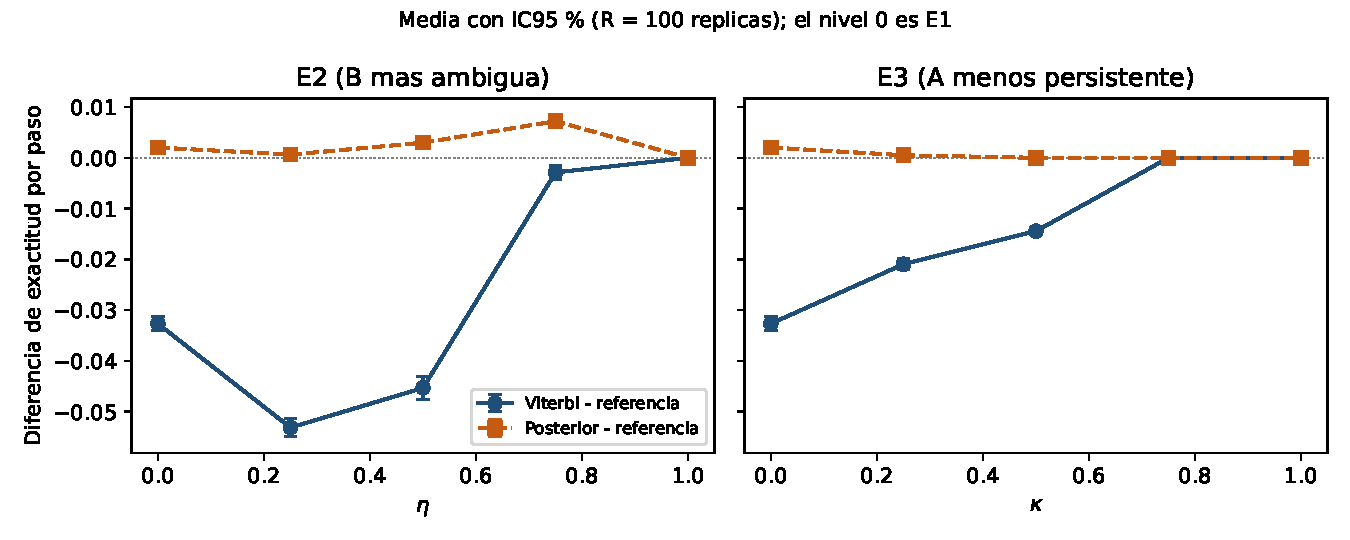
\includegraphics[width=\textwidth]{results/fig_D.pdf}
\caption{Media de $D=\mathrm{Acc}^{\mathrm{Vit}}-\mathrm{Acc}^{\mathrm{ref}}$ y de
$D_{\mathrm{post}}=\mathrm{Acc}^{\mathrm{post}}-\mathrm{Acc}^{\mathrm{ref}}$ con
IC95\,\% frente a $\eta$ (E2) y $\kappa$ (E3). El nivel 0 corresponde a E1.}
\label{fig:D}
\end{figure}

\subsection{Descripción de lo observado}

\begin{itemize}
\item \textbf{E1.} La exactitud media por paso fue $0.518$ con Viterbi y
$0.551$ con el clasificador de referencia: $\bar D=-0.033$, IC95\,\%
$[-0.034,\,-0.031]$. Por fase, Viterbi acertó más en defensiva ($0.810$ frente a
$0.701$) y en ataque ($0.430$ frente a $0.399$), y menos en transición
($0.251$ frente a $0.500$).
\item \textbf{E2.} $\bar D$ fue negativa en $\eta=0.25$, $0.5$ y $0.75$, con su
valor más bajo en $\eta=0.25$ ($-0.053$). Desde $\eta=0.75$, Viterbi asignó
``defensiva'' a todos los pasos; el clasificador de referencia dejó de asignar
``ataque'' en $\eta=0.75$, como se había anticipado. En $\eta=1$ ambos métodos
asignaron ``defensiva'' a todos los pasos y $D=0$ en todas las réplicas.
\item \textbf{E3.} $\bar D$ aumentó hacia 0 al crecer $\kappa$: $-0.021$
($\kappa=0.25$) y $-0.014$ ($\kappa=0.5$). En $\kappa=0.75$ y $\kappa=1$ ambos
métodos produjeron exactamente las mismas asignaciones en todas las réplicas
($D=0$, $s_D=0$).
\item \textbf{Decodificación posterior.} $\bar D_{\mathrm{post}}$ fue positiva
pero pequeña en E1 ($+0.0020$, IC95\,\% $[+0.0016,\,+0.0025]$), en
$\eta=0.25$, $0.5$ y $0.75$ (máximo en $\eta=0.75$: $+0.0072$) y en
$\kappa=0.25$ ($+0.0005$). Fue exactamente 0 en $\eta=1$ y en
$\kappa\ge0.5$. En ninguna configuración fue negativa. En E1, su exactitud por
fase fue $0.690$ (defensiva), $0.493$ (transición) y $0.432$ (ataque), cercana a
la del clasificador de referencia salvo en ataque.
\item \textbf{Controles negativos.} Se cumplieron para los tres métodos: $D=0$
y $D_{\mathrm{post}}=0$ en $\eta=1$ y en $\kappa=1$. Los resultados $D=0$ en
$\kappa=0.75$ y $D_{\mathrm{post}}=0$ en $\kappa=0.5$ no se habían anticipado.
\end{itemize}

\subsection{Verificación complementaria}

Al observar que en E1 Viterbi era menos exacto que el clasificador de
referencia, y antes de añadir la decodificación posterior al diseño, se ejecutó
un diagnóstico (\path{verificacion/diagnostico_decodificacion.py}, con
semillas distintas): (i) la exactitud esperada del clasificador de referencia,
calculada analíticamente como $\sum_o\max_i p_i b_i(o)$, es $0.550$, coherente
con el $0.551$ observado; (ii) Viterbi coincidió con la búsqueda exhaustiva en
100 de 100 secuencias simuladas de E1 con $T=8$; (iii) en 2000 secuencias de
E1, la exactitud media fue $0.5548$ (posterior), $0.5516$ (referencia) y
$0.5221$ (Viterbi). Junto con la Tabla~\ref{tab:res}, estos datos indican que
la menor exactitud por paso de Viterbi no se debe a un error de implementación:
Viterbi maximiza la probabilidad del camino completo, no el número esperado de
pasos acertados.

% ------------------------------------------------------------
\section{Discusión}

\subsection{Síntesis de los hallazgos}

Con los parámetros hipotéticos del caso, usar las transiciones no mejoró la
exactitud por paso de Viterbi: fue $0.033$ menor que la del clasificador sin
transiciones. La decodificación posterior, que usa las mismas transiciones pero
elige la fase más probable en cada paso, sí superó al clasificador, aunque solo
por $0.002$. Al hacer más ambiguas las emisiones, la pérdida de Viterbi no
varió de forma constante (fue máxima en $\eta=0.25$) y, desde $\eta=0.75$,
Viterbi asignó una única fase a todos los pasos. Al reducir la persistencia de
las transiciones, los tres métodos dejaron de diferir a partir de un nivel
($\kappa=0.75$ para Viterbi y $\kappa=0.5$ para la decodificación posterior):
la convergencia no fue gradual, sino que las asignaciones pasaron a ser
idénticas.

Como se indicó en la sección~5.2, el hecho de que Viterbi resulte menos exacto
por paso no se debe a un error de implementación: Viterbi maximiza la
probabilidad del camino completo, mientras que la métrica empleada premia el
número de pasos acertados.

Además, los resultados son compatibles con dos explicaciones que este diseño
no permite confirmar y que se plantean como hipótesis:

\begin{enumerate}[label=\textbf{(\alph*)}, leftmargin=*]
  \item \textbf{Solapamiento de las emisiones.} Las tres fases emiten con
  frecuencia las mismas acciones: el pase corto tiene probabilidad
  $0.70$, $0.40$ y $0.30$ en defensiva, transición y ataque, y ni siquiera
  en ataque el tiro supera $0.40$. Si una acción apenas identifica su fase,
  ningún método puede acertar mucho, lo que es compatible con que la
  exactitud no superara $0.56$ en ninguna configuración. En E2, al aumentar
  el solapamiento, la exactitud de la referencia bajó de $0.551$ a $0.393$
  ($\eta=0.75$) y la ventaja de la decodificación posterior creció hasta
  $0.007$. Esta hipótesis explica el nivel general de exactitud, pero no por
  qué Viterbi queda por debajo de la referencia, ya que el solapamiento
  afecta a los tres métodos.

  \item \textbf{Sesgo de Viterbi hacia la fase más persistente y frecuente.}
  En E1, Viterbi asignó la fase defensiva al 62\,\% de los pasos, frente al
  39\,\% en que esa fase fue la verdadera (49\,\% en la referencia y
  47\,\% en la decodificación posterior; Tabla~\ref{tab:conf}). Acertó el
  81\,\% de los pasos defensivos, pero solo el 25\,\% de los de
  transición, frente al 50\,\% de la referencia (Tabla~\ref{tab:fase}). Al
  aumentar $\eta$, su acierto en la fase defensiva subió a $0.86$, $0.97$ y
  $1.00$. Esto es compatible con que el criterio de camino completo favorezca
  permanecer en la fase con mayor probabilidad de permanencia ($a_{11}=0.60$)
  y mayor frecuencia estacionaria ($0.389$). Como en este modelo ambas
  propiedades coinciden en la misma fase, los datos no permiten separar cuál
  de las dos produce el sesgo.
\end{enumerate}

\subsection{Relación con las fuentes}

Ötting et al.\ advierten que, en un ajuste no supervisado, los estados de un
HMM son solo aproximaciones de estados genuinos \cite[p.~23]{otting2023}. En
este trabajo la situación es la más favorable posible (modelo correctamente
especificado y parámetros conocidos) y, aun así, la exactitud por paso no
superó $0.56$ en ninguna configuración. Este resultado es coherente con esa
advertencia, aunque no la prueba para datos reales.

Fani et al.\ informan una exactitud del 98,7\,\% en la segmentación
juego/interrupción \cite[p.~27322]{fani2017}. Esa cifra no es comparable con
las de este trabajo: los datos, las observaciones, el número de estados y el
procedimiento de evaluación son distintos.

\subsection{Limitaciones}

\begin{enumerate}
\item Los resultados valen solo para el modelo simulado con los parámetros
hipotéticos del caso y las variaciones E2--E3; no permiten afirmar nada sobre
partidos reales.
\item El modelo está correctamente especificado por construcción, condición que
no se cumple con datos reales \cite[p.~23]{otting2023}.
\item Las exactitudes no son comparables con las de \cite{fani2017}.
\item Se evaluó un único conjunto de parámetros base, una única longitud de
secuencia ($T=100$) y una única métrica principal (exactitud por paso), que
favorece por definición a la decodificación posterior frente a Viterbi.
\end{enumerate}

% ------------------------------------------------------------
\section{Conclusiones y trabajo futuro}\label{sec:conclusiones}

\begin{description}[leftmargin=1.2cm]
\item[P1:] No. Con los parámetros del caso, Viterbi fue menos exacto por paso
que el clasificador sin transiciones ($\bar D=-0.033$; IC95\,\%
$[-0.034,\,-0.031]$). La decodificación posterior sí lo superó, pero la
diferencia fue de dos milésimas ($\bar D_{\mathrm{post}}=+0.002$; IC95\,\%
$[+0.0016,\,+0.0025]$).
\item[P2:] Con emisiones más ambiguas, la diferencia de Viterbi fue negativa en
todos los niveles intermedios y no varió de forma constante: fue máxima en
$\eta=0.25$ ($-0.053$) y se acercó a 0 en niveles altos, donde Viterbi asignó
una única fase (defensiva) a todos los pasos.
\item[P3:] Al reducir la persistencia de las transiciones, los tres métodos
convergieron y produjeron asignaciones idénticas desde $\kappa=0.75$
($D=0$); la decodificación posterior coincidió con el clasificador ya desde
$\kappa=0.5$.
\end{description}

Estas respuestas se limitan al modelo simulado; no permiten afirmaciones sobre
partidos reales.

\textbf{Trabajo futuro.} (i) Estimar los parámetros con Baum--Welch y comparar
con los verdaderos; (ii) definir operativamente las fases y buscar datos reales
con licencia adecuada; si las fases pudieran anotarse, como los estados
juego/interrupción de \cite{fani2017}, sería posible medir exactitud con datos
reales usando una partición entrenamiento/prueba por partidos; (iii) explorar observaciones más ricas, como las
variables minuto a minuto de \cite{otting2023}.

% ------------------------------------------------------------
\section*{Declaración de uso de inteligencia artificial}
Se usó un asistente de
IA (Claude, Anthropic) para estructurar el documento según la plantilla,
redactar borradores, extraer el texto de las fuentes, escribir y verificar el
código, y ejecutar la simulación. Las decisiones de alcance, preguntas,
escenarios, valores del diseño, métodos, fuentes, semilla y autoría
fueron tomadas por el equipo, que es responsable del contenido.

% ------------------------------------------------------------
\begin{thebibliography}{9}
\bibitem{otting2023}
M.~Ötting, R.~Langrock y A.~Maruotti, ``A copula-based multivariate hidden
Markov model for modelling momentum in football,'' \emph{AStA Advances in
Statistical Analysis}, vol.~107, pp.~9--27, 2023.
doi:\href{https://doi.org/10.1007/s10182-021-00395-8}{10.1007/s10182-021-00395-8}.

\bibitem{fani2017}
M.~Fani, M.~Yazdi, D.~A.~Clausi y A.~Wong, ``Soccer video structure analysis
by parallel feature fusion network and hidden-to-observable transferring Markov
model,'' \emph{IEEE Access}, vol.~5, pp.~27322--27336, 2017.
doi:\href{https://doi.org/10.1109/ACCESS.2017.2769140}{10.1109/ACCESS.2017.2769140}.
\end{thebibliography}

% ------------------------------------------------------------
\appendix
\section*{Anexo A: estructura de la carpeta del proyecto}
El proyecto es un repositorio Git local; las instrucciones para reproducir los
resultados están en \texttt{README.md}.
\begin{verbatim}
/anteproyecto-futbol
    README.md                 descripcion e instrucciones
    main.tex, main.pdf        este manuscrito
    bitacora.md               decisiones y verificaciones
    requirements.txt          versiones usadas
    main_simulation.py        ejecuta E1-E3 y exporta CSV
    figuras.py                genera results/fig_D.pdf
    tablas_latex.py           genera results/tablas_resultados.tex
    /src
        hmm_core.py           viterbi_log, posterior_decode,
                              clasificador_ref, simular
        utils_stats.py        media, desviacion, IC95 %
    /verificacion
        diagnostico_decodificacion.py
        test_posterior.py
    /results                  CSV, figura, tablas, entorno.txt,
                              salidas de verificacion
        /ejecucion1           archivo de la primera ejecucion
\end{verbatim}

\section*{Anexo B: guion del vídeo (2--3 minutos)}
\begin{enumerate}
\item \textbf{0:00--0:30.} Problema: la fase táctica no se observa; preguntas P1--P3.
\item \textbf{0:30--1:30.} Modelo $\lambda$ del caso, clasificador de referencia y diseño E1--E3.
\item \textbf{1:30--2:20.} Resultados (en pantalla: Tabla~\ref{tab:res} y
Figura~\ref{fig:D}). Con los parámetros del caso, Viterbi acierta menos que el
clasificador sin transiciones ($\bar D=-0.033$), mientras que la decodificación
posterior lo supera por solo $0.002$. No es un error de código: Viterbi busca
el camino completo más probable, no el mayor número de pasos acertados. Con
emisiones más ambiguas (E2), Viterbi termina asignando la fase defensiva a
todos los pasos; con transiciones menos persistentes (E3), los tres métodos
acaban dando las mismas asignaciones. En pantalla, la matriz de confusión
(Tabla~\ref{tab:conf}): Viterbi asigna defensiva al 62\,\% de los pasos,
cuando la verdad es el 39\,\%.
\item \textbf{2:20--2:50.} Conclusión y límites. Con estos parámetros, usar
las transiciones aporta poco a la exactitud por paso, y con Viterbi incluso la
reduce. Dos hipótesis compatibles con los datos: las acciones se parecen entre
fases y Viterbi se inclina hacia la fase más persistente y frecuente. Los
resultados valen solo para el modelo simulado, con parámetros conocidos, y no
permiten afirmaciones sobre partidos reales.
\end{enumerate}

\end{document}
